% !TeX root = proposal.tex
\chapter{Evaluate the Household IoT Privacy-setting Interface Prototype (Proposed work)}\label{chapter:evaluation}

\section{Introduction}

In the previous chapters, we have described the three studies on recommending privacy settings for general/public IoT, household IoT, and fitness IoT, respectively. A ``data-driven” approach has been used in all three studies, to gain the underlying insights of IoT users' privacy decision behavior, and to design a set of interfaces to incorporate the ``smart" privacy default/profiles created based on the insights. Users can apply these smart defaults/profiles by either a single click or by answering a few related questions. When applying this approach on the household IoT dataset in Chapter~\ref{chapter:householdIoT}, we explored the trade-off between parsimony and accuracy when creating the ``smart" privacy defaults/profiles. We manipulate the pruning parameter for the decision trees of the C4.5 algorithm, which impacted the complexity of the generated profiles based on the decision trees. Accuracy is important to ensure that users' privacy preferences are accurately captured and/or need only few manual adjustments, while parsimony, on the other hand, prevents overfitting and promotes fairness. In Chapter~\ref{chapter:householdIoT}, we noticed that more complex models tended to increase overall accuracy by predicting a few users' preferences more accurately, with no effect on other users. Parsimony also makes the associated default setting easier to understand for the user. 

The biggest limitation of our work so far is that we did not test any of the proposed interfaces, so we do not know what level of complexity (both in terms of the user interface and the in terms of the profiles) is most suitable. Thus, to further test this trade-off between accuracy and parsimony in a real usage environment and test the user experience of using the interfaces that we designed in Chapter~\ref{chapter:householdIoT}, for my proposed work, I will address this limitation by discussing our proposed study to evaluate the new interface prototypes of recommending privacy-settings for household IoT. The main purpose of this proposed work is to test the user experience of the privacy-setting interfaces.

In this chapter, we first discuss the design of our evaluation system, then we present my proposed study plan, including how we recruit participants for our study, our experimental design, how we measure our results, and expected results.

\section{Study Design}


In this section, we discuss the experimental design of our user study. This proposed user study will be a between-subject study, which takes about 15 -- 20 minutes to finish. All participants will be recruited via Amazon Mechanical Turk.

\subsection{Dependent Variables}
Since we want to test the user experience when they use our privacy-setting interfaces and , the Dependent Variable of our study will be the user experience of the system. 

\subsection{Independent Variables}
In Chapter~\ref{chapter:householdIoT},  we first designed a set of interfaces, as shown in Figure~\ref{fig:interface2}, based on the results from our statistical analysis (\textbf{UI1}). Further, we modified these interfaces to integrate the ``smart defaults/profiles" generated from our machine learning results. This modification separated the Storage and sharing modules from the Data usage, leading a more complex interface design (\textbf{UI2}). For our study, we need to test these two groups of interfaces (UI1 vs UI2) in terms of interface complexity.

In terms of the complexity of ``smart defaults/profiles", we consider 4 different experimental conditions as follows:
\begin{itemize}
	\item \textbf{Everything-Off}: With all the data access and usage being turned off, this is considered as the most simple and conservative default settings.
	\item \textbf{Everything-On}: With all the data access and usage being turned on, this is considered as the most simple and open default settings.
	\item \textbf{Smart Default}: One single ``smart profile" will be provided to the users. This is considered as the experimental condition with intermediate complexity.
	\item \textbf{Smart Profiles}: Multiple ``smart profiles" will be provided to the users. This is considered as the most sophisticated settings with high complexity in ``smart profiles".
\end{itemize}

These different default/profile conditions map to users' ``preference fit", where the smart profile have a better preference fit than the smart default, which in turn has a better fit than Everything-Off/Everything On defaults.

From above, we have 2 different levels of interface complexity, and 4 different levels of profile complexity.
Hence, $4$x$2=8$ total experimental conditions (i.e., user interfaces) will be presented to the participants. 

\subsection{Profile/Interface Selection}
\textbf{Everything-Off} and \textbf{Everything On} profiles can easily be implemented on both our designed interfaces (UI1 and UI2).

For \textbf{Smart Default} and \textbf{Smart Profiles} selection, noted that, when applying our machine learning algorithms in Chapter~\ref{chapter:householdIoT}, we have manipulated the pruning parameter to create different ``smart defaults/profiles". This manipulation results in a set of smart profiles with different weight in accuracy and parsimony. The more the decision tree is pruned, the less complex the resulting ``smart" profile will be, leading lower accuracy and high parsimony, and vice versa. Since we can only choose one ``smart default/profile" to test the interface, this selection needs to be done carefully.

\textbf{Smart Default:} In section~\ref{subsection:onerule2}, we have applied a one-rule algorithm to our dataset. The resulting ``smart default" in shown in Figure~\ref{fig:oneR}. This is the simplest ``smart default" settings across all the different ``smart defaults" settings with lowest accuracy (61.39\%) but highest parsimony. In addition, this ``smart default" can be easily integrate into the \textbf{UI1}, the simpler interfaces. Thus, we choose this ``smart default" as the target interface for experimental condition --- \textbf{UI1:Smart Default}. In contrast, we created a ``smart default" setting with only 8 nodes shown in Figure~\ref{fig:smart_default_new} in section~\ref{subsection:overall2}. This ``smart default" has the very high parsimony and the close to highest accuracy of 63.32\% across all the ``smart default" settings. In addition, this ``smart default" can be easily integrate into the \textbf{UI2}, the simpler interfaces. Thus, we choose this ``smart default" as the target interface for experimental condition --- \textbf{UI2:Smart Default}.

\textbf{Smart Profiles:} For ``smart profiles" selection, we want this interface differ as much as possible comparing the ``smart default", so we search across all the ``smart profiles" with large number of clusters. In addition, the ``smart profiles" should be easily integrated into UI1 or UI2. Figure~\ref{fig:conglo_5_profile001} is considered for UI1 because it has 5 clusters with a high accuracy of 80.35\%. And it has no interaction between \textbf{Storage} and other parameters. This is suitable for our UI1 design, serving as the target interface profiles for experimental condition --- \textbf{UI1:Smart Profiles}. We have separated the Data Storage and Data Usage modules in UI2. Thus, we choose Figure~\ref{fig:fit_5_profile003} for UI2 because it has 5 clusters, a close to highest accuracy of 83.11\%. In addition, in the cluster 3, it has a 2-way interaction between \textbf{Storage} and \textbf{Purpose}; in cluster 4, it has a 2-way interaction between \textbf{Storage} and \textbf{Action}. It does not have an 3-way interaction between any of these parameters in any of its clusters. Thus, we choose this set of ``smart profiles" as the target interface profiles for experimental condition --- \textbf{UI2:Smart Profiles}.


\subsection{Interfaces Implementation}
We have implemented above 8 different sets of user interfaces using HTML, PHP, CSS, and SQL. Figure~\ref{fig:ui1AllOff} shows the experimental condition --- UI1:Everything-Off.
\begin{figure}
	\centering
	\begin{subfigure}[t]{0.24\textwidth}
		\centering
		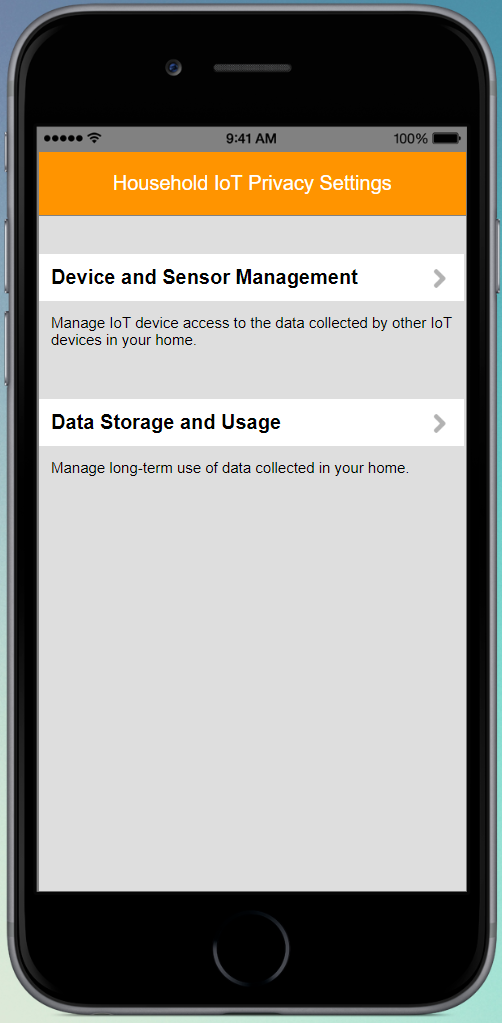
\includegraphics[height=2.8in]{figures/ui1allOff1.png}
	\end{subfigure}%
	~
	\begin{subfigure}[t]{0.24\textwidth}
		\centering
		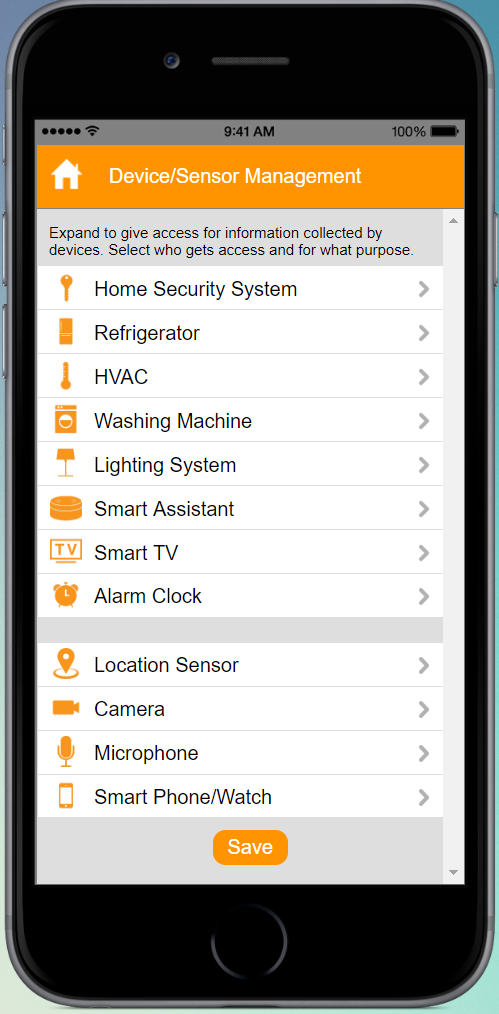
\includegraphics[height=2.8in]{figures/ui1allOff2.png}
	\end{subfigure}%
	~
	\begin{subfigure}[t]{0.24\textwidth}
		\centering
		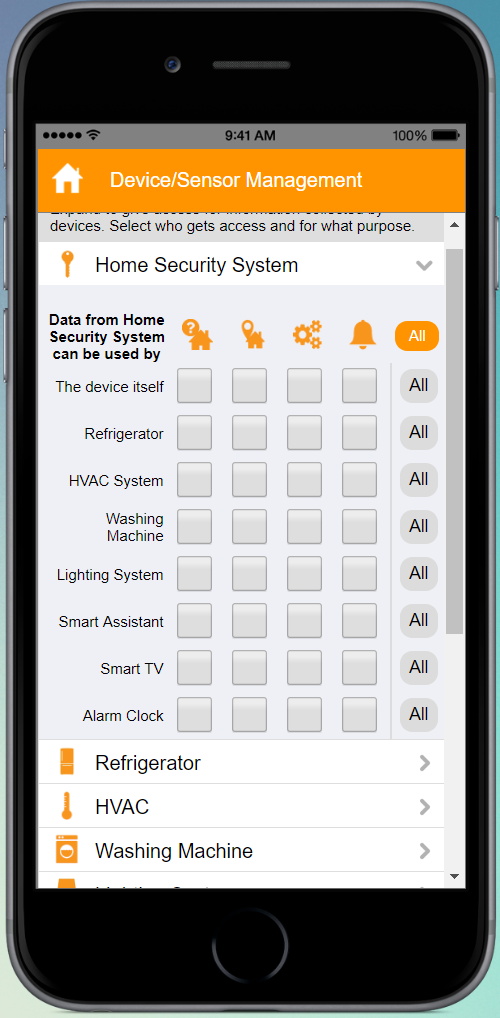
\includegraphics[height=2.8in]{figures/ui2allOff3.png}
	\end{subfigure}%
	~
	\begin{subfigure}[t]{0.24\textwidth}
		\centering
		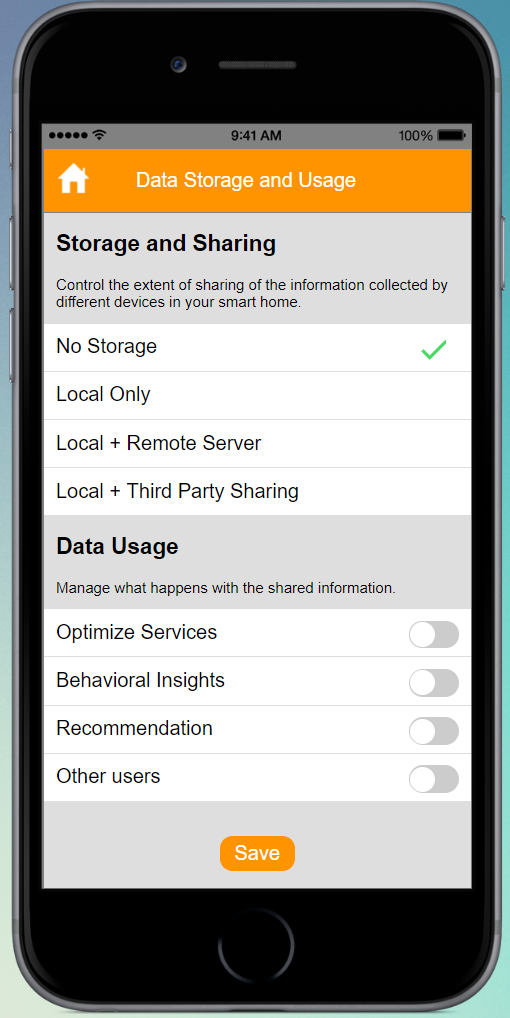
\includegraphics[height=2.8in]{figures/ui1allOff4.png}
	\end{subfigure}%
	\caption{User Interface 1 with all settings turned off}
	\label{fig:ui1AllOff}
\end{figure}

Figure~\ref{fig:ui2AllOff} shows the experimental condition --- UI2:Everything-Off.
\begin{figure}
	\centering
	\begin{subfigure}[t]{0.2\textwidth}
		\centering
		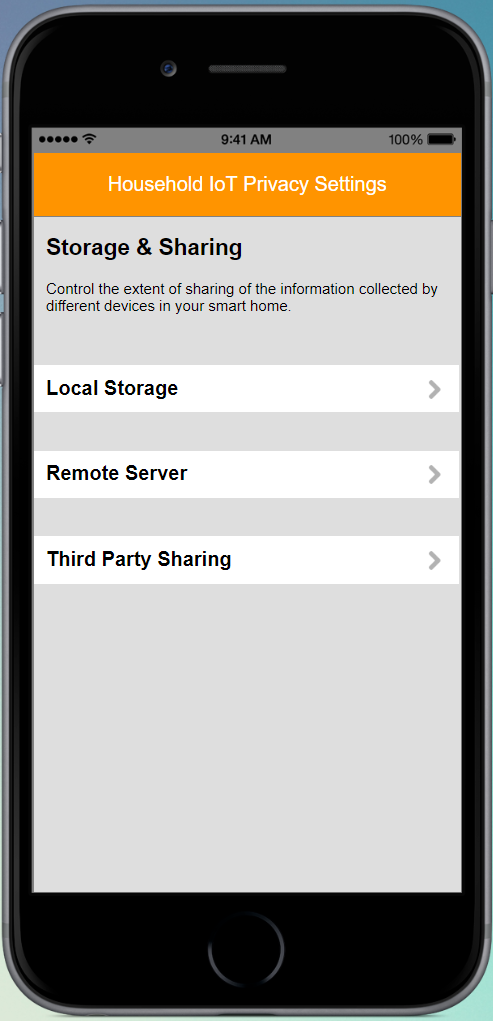
\includegraphics[height=2.8in]{figures/ui2allOff1.png}
	\end{subfigure}%
	~~~~~
	\begin{subfigure}[t]{0.2\textwidth}
	\centering
	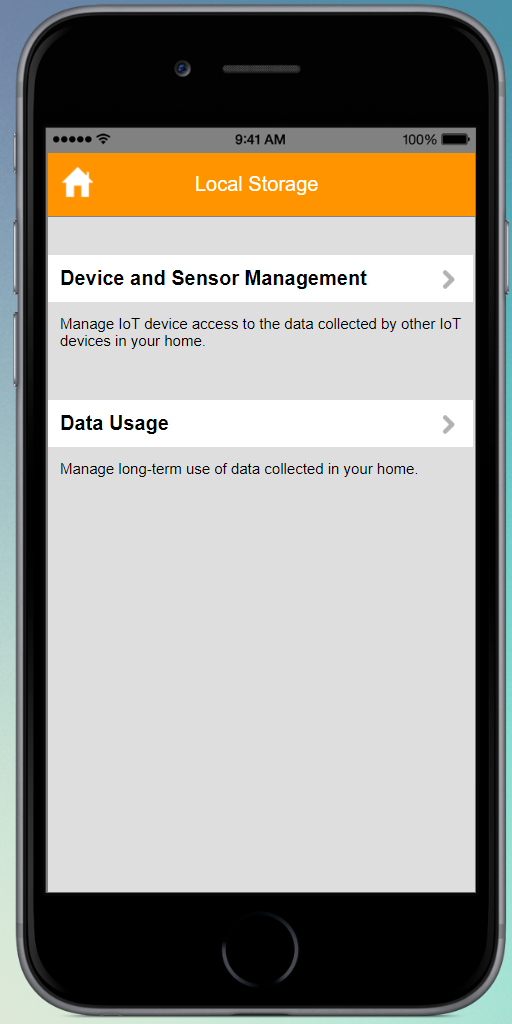
\includegraphics[height=2.8in]{figures/ui2allOffLocal.png}
	\end{subfigure}%
	~~~~~
	\begin{subfigure}[t]{0.2\textwidth}
		\centering
		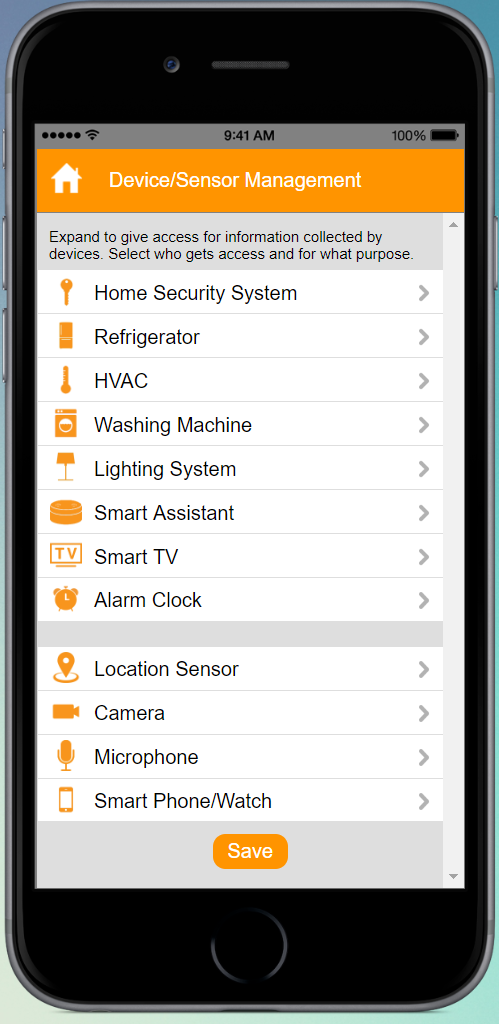
\includegraphics[height=2.8in]{figures/ui2allOff2.png}
	\end{subfigure}%
	~~~~~
	\begin{subfigure}[t]{0.2\textwidth}
		\centering
		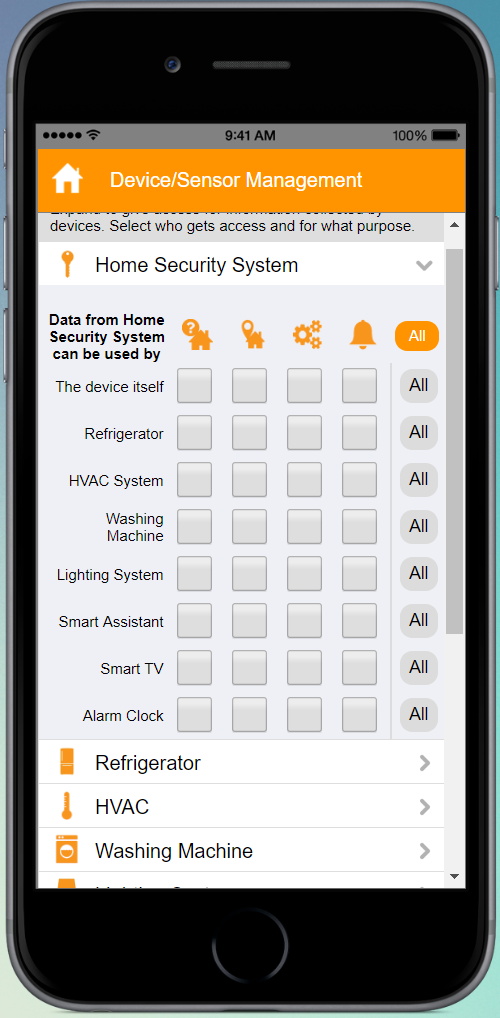
\includegraphics[height=2.8in]{figures/ui2allOff3.png}
	\end{subfigure}%
	~~~~~
	\begin{subfigure}[t]{0.2\textwidth}
		\centering
		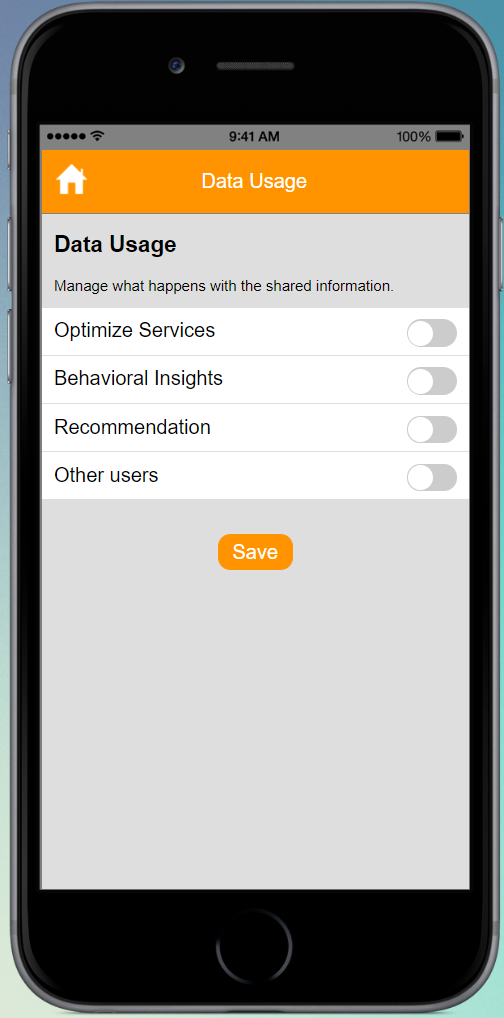
\includegraphics[height=2.8in]{figures/ui2allOff4.png}
	\end{subfigure}%
	\caption{User Interface 2 with all settings turned off}
	\label{fig:ui2AllOff}
\end{figure}

Figure~\ref{fig:ui1AllOn} shows the experimental condition --- UI1:Everything-On.
\begin{figure}
	\centering
	\begin{subfigure}[t]{0.24\textwidth}
		\centering
		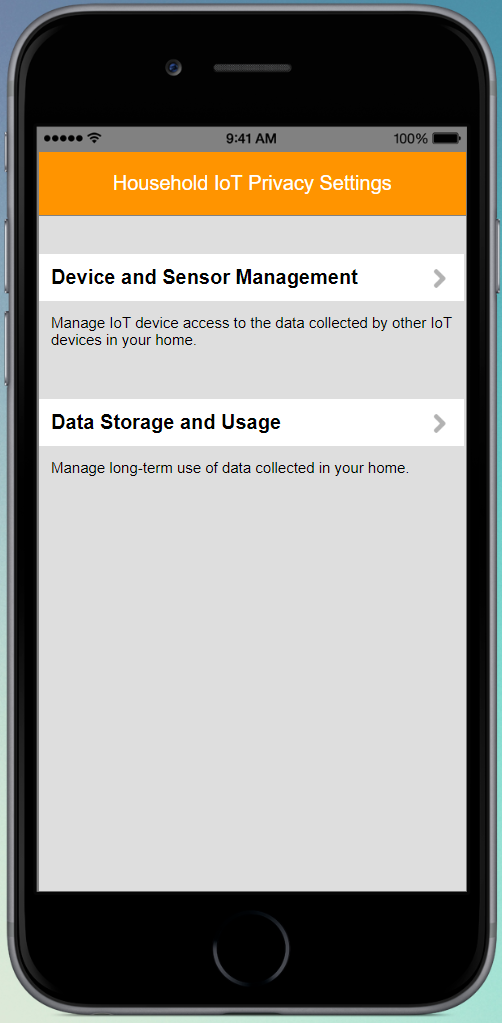
\includegraphics[height=2.8in]{figures/ui1allOff1.png}
	\end{subfigure}%
	~
	\begin{subfigure}[t]{0.24\textwidth}
		\centering
		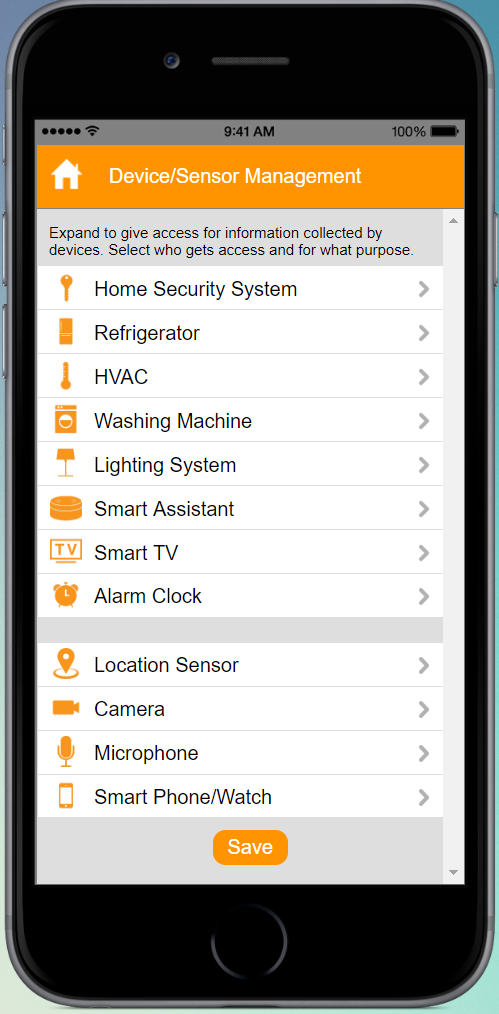
\includegraphics[height=2.8in]{figures/ui1allOff2.png}
	\end{subfigure}%
	~
	\begin{subfigure}[t]{0.24\textwidth}
		\centering
		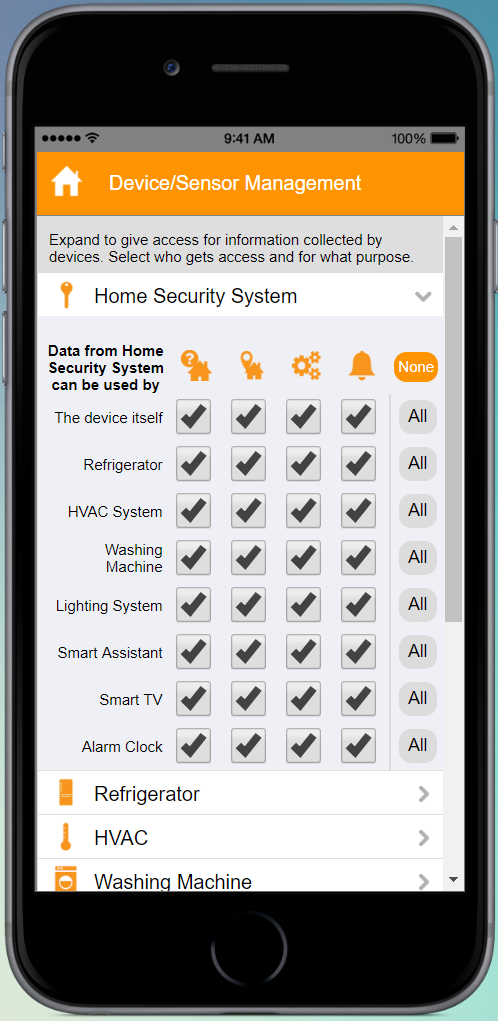
\includegraphics[height=2.8in]{figures/ui2allOn3.png}
	\end{subfigure}%
	~
	\begin{subfigure}[t]{0.24\textwidth}
		\centering
		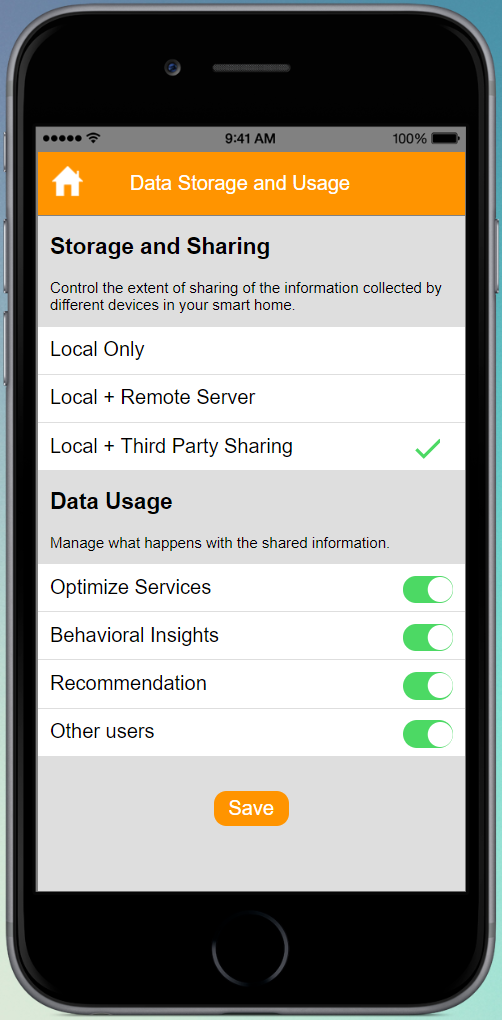
\includegraphics[height=2.8in]{figures/ui1allOn4.png}
	\end{subfigure}%
	\caption{User Interface 1 with all settings turned on}
	\label{fig:ui1AllOn}
\end{figure}

Figure~\ref{fig:ui2AllOn} shows the experimental condition --- UI2:Everything-On.
\begin{figure}
	\centering
	\begin{subfigure}[t]{0.19\textwidth}
		\centering
		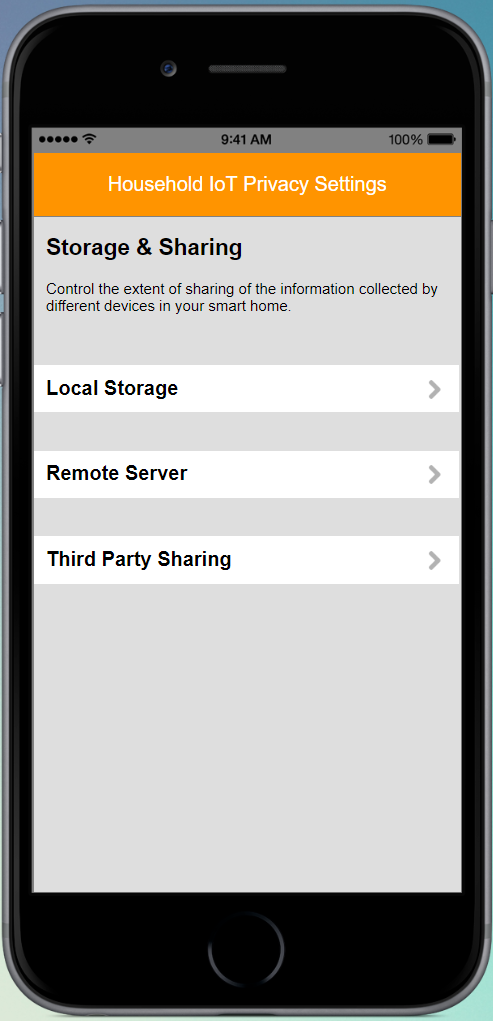
\includegraphics[height=2.8in]{figures/ui2allOff1.png}
	\end{subfigure}%
	~~~~~~
	\begin{subfigure}[t]{0.19\textwidth}
	\centering
	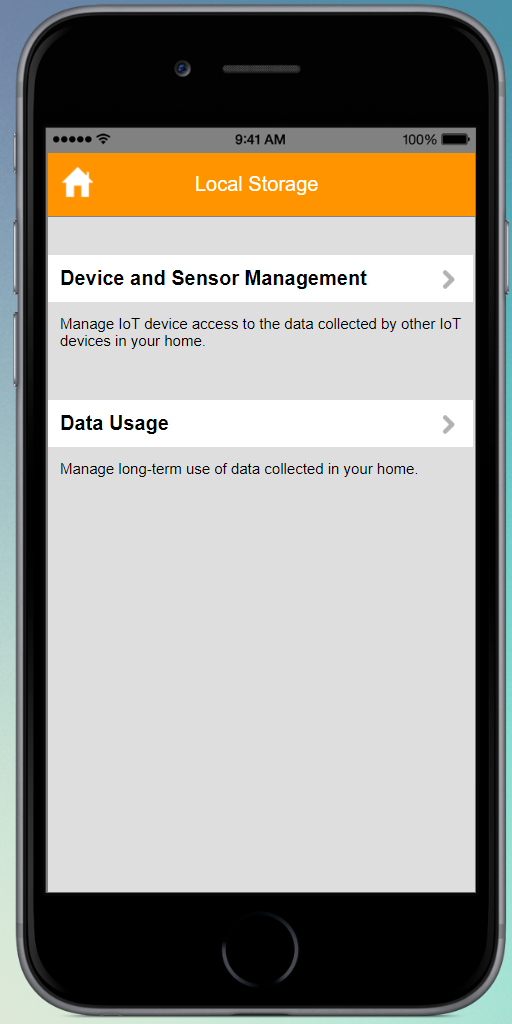
\includegraphics[height=2.8in]{figures/ui2allOffLocal.png}
	\end{subfigure}%
	~~~~~~
	\begin{subfigure}[t]{0.19\textwidth}
		\centering
		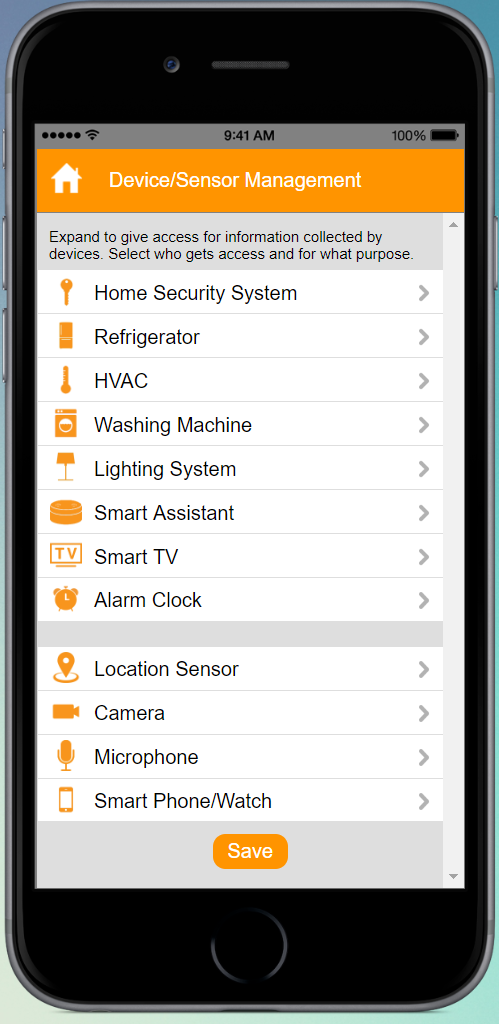
\includegraphics[height=2.8in]{figures/ui2allOff2.png}
	\end{subfigure}%
	~~~~~~
	\begin{subfigure}[t]{0.19\textwidth}
		\centering
		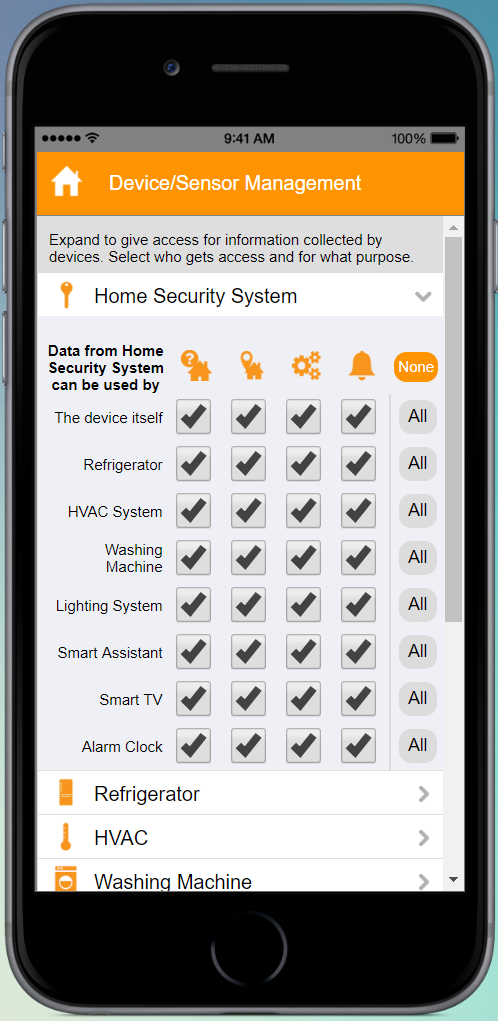
\includegraphics[height=2.8in]{figures/ui2allOn3.png}
	\end{subfigure}%
	~~~~~~
	\begin{subfigure}[t]{0.19\textwidth}
		\centering
		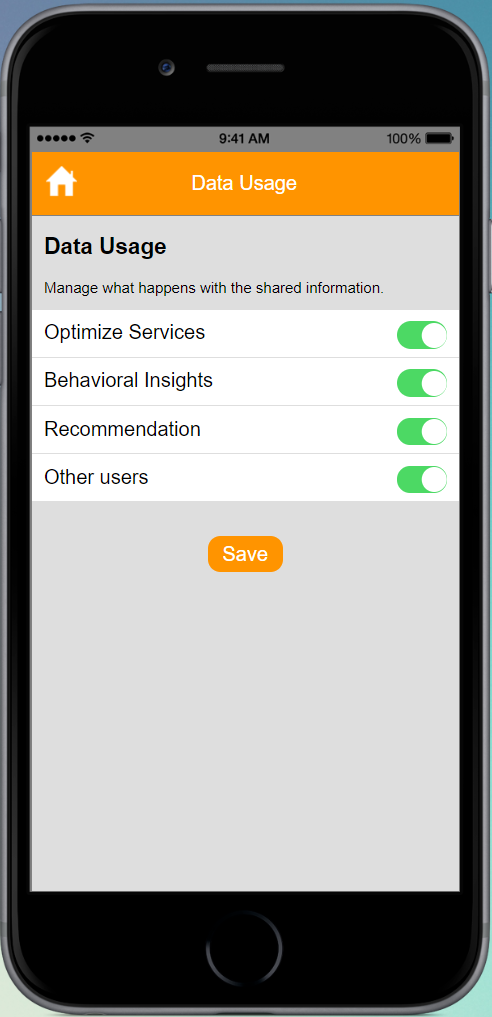
\includegraphics[height=2.8in]{figures/ui2allOn4.png}
	\end{subfigure}%
	\caption{User Interface 2 with all settings turned on}
	\label{fig:ui2AllOn}
\end{figure}

Figure~\ref{fig:ui1OneR} shows the experimental condition --- UI1:Smart Default.
\begin{figure}
	\centering
	\begin{subfigure}[t]{0.24\textwidth}
		\centering
		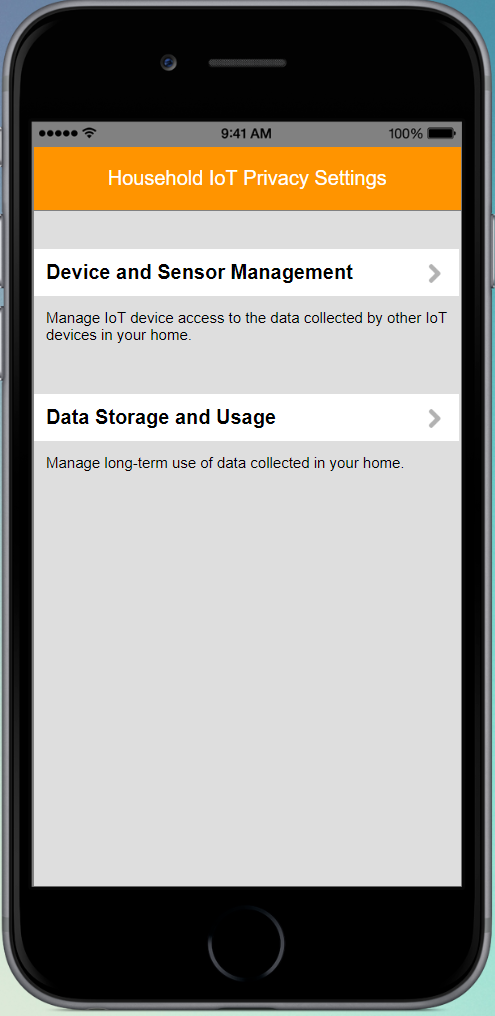
\includegraphics[height=2.8in]{figures/ui1sd1.png}
	\end{subfigure}%
	~
	\begin{subfigure}[t]{0.24\textwidth}
		\centering
		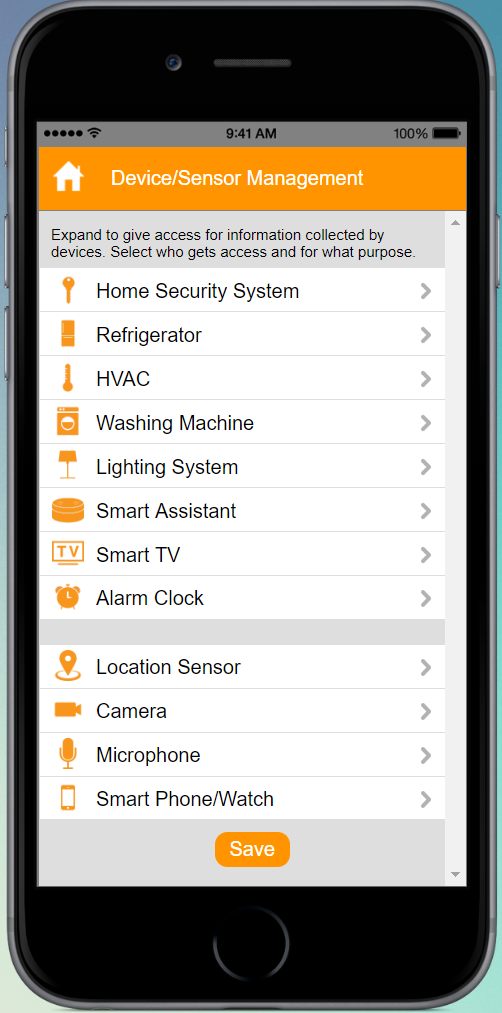
\includegraphics[height=2.8in]{figures/ui1sd2.png}
	\end{subfigure}%
	~
	\begin{subfigure}[t]{0.24\textwidth}
		\centering
		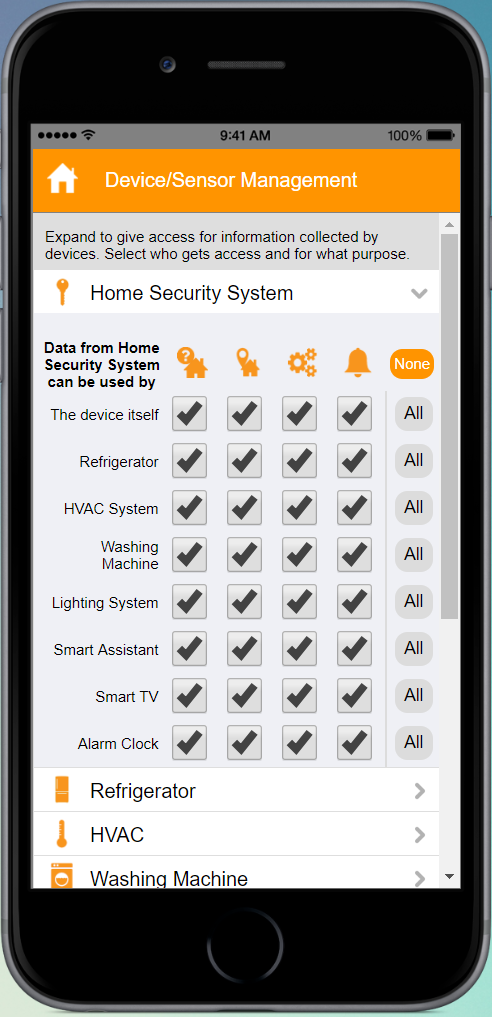
\includegraphics[height=2.8in]{figures/ui1sd3.png}
	\end{subfigure}%
	~
	\begin{subfigure}[t]{0.24\textwidth}
		\centering
		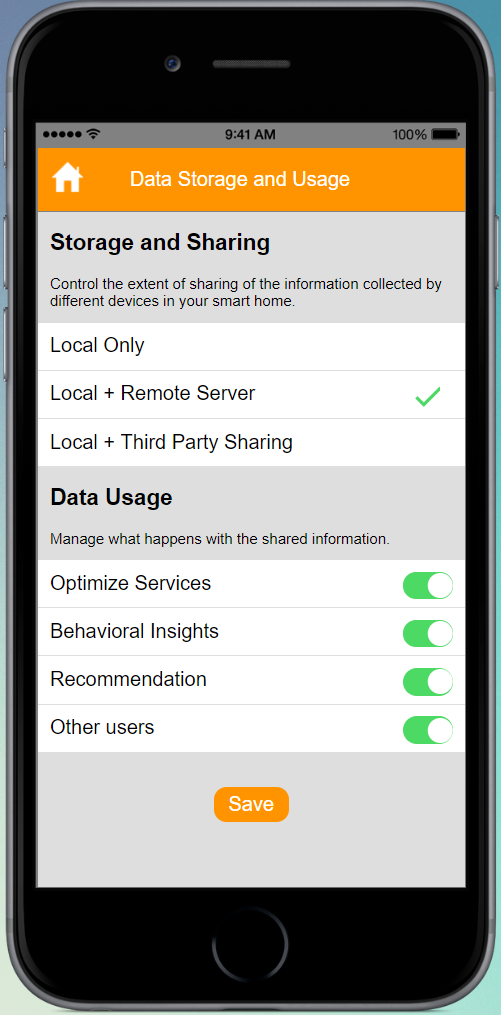
\includegraphics[height=2.8in]{figures/ui1sd4.png}
	\end{subfigure}%
	\caption{User Interface 1 with Smart Default}
	\label{fig:ui1OneR}
\end{figure}

Figure~\ref{fig:ui2SD} shows the experimental condition --- UI2:Smart Default.
\begin{figure}
	\centering
	\begin{subfigure}[t]{0.2\textwidth}
	\centering
	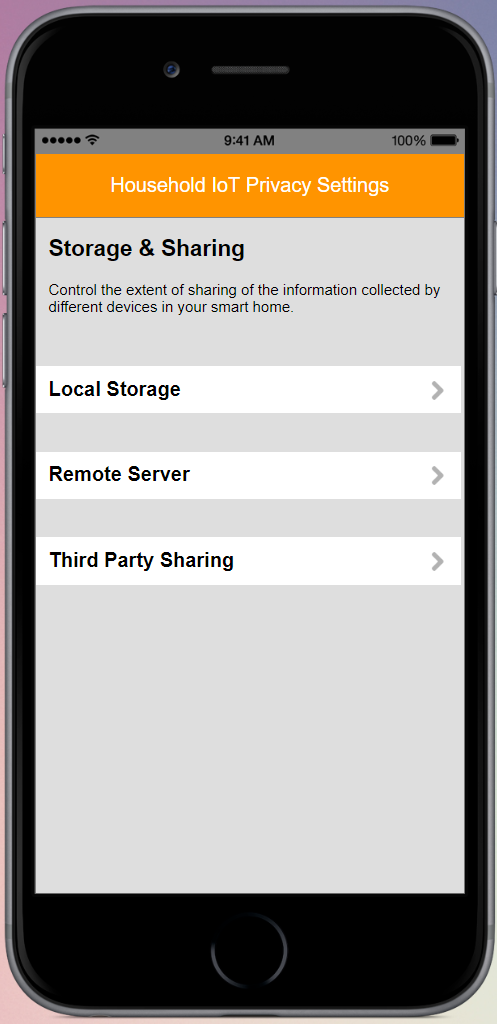
\includegraphics[height=2.8in]{figures/ui2sd1.png}
	\end{subfigure}%
	~~~~~
	\begin{subfigure}[t]{0.2\textwidth}
		\centering
		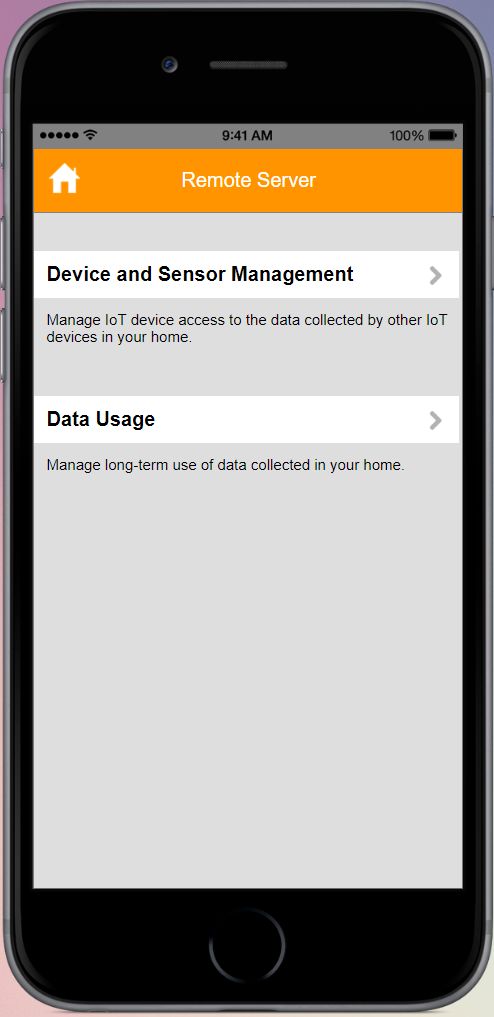
\includegraphics[height=2.8in]{figures/ui2sd2.png}
	\end{subfigure}%
	~~~~~
	\begin{subfigure}[t]{0.2\textwidth}
		\centering
		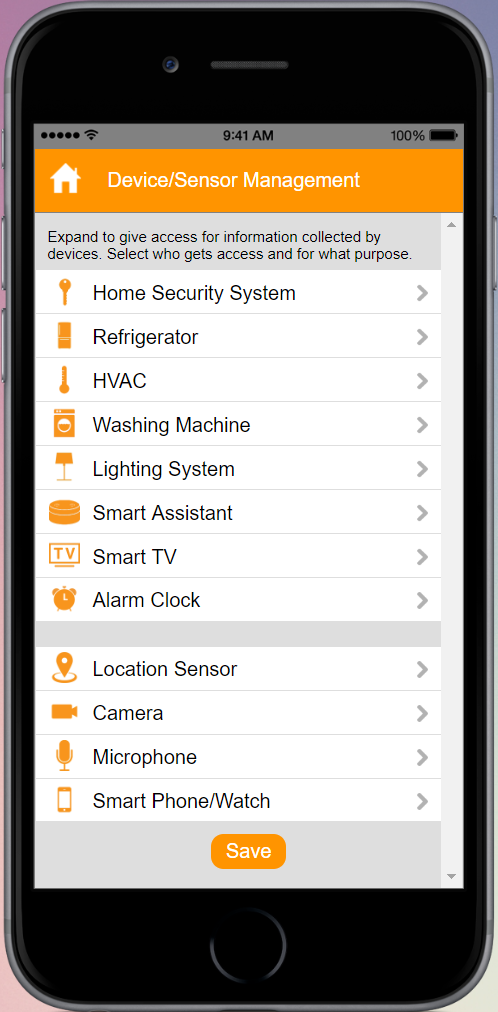
\includegraphics[height=2.8in]{figures/ui2sd3.png}
	\end{subfigure}%
	~~~~~
	\begin{subfigure}[t]{0.2\textwidth}
		\centering
		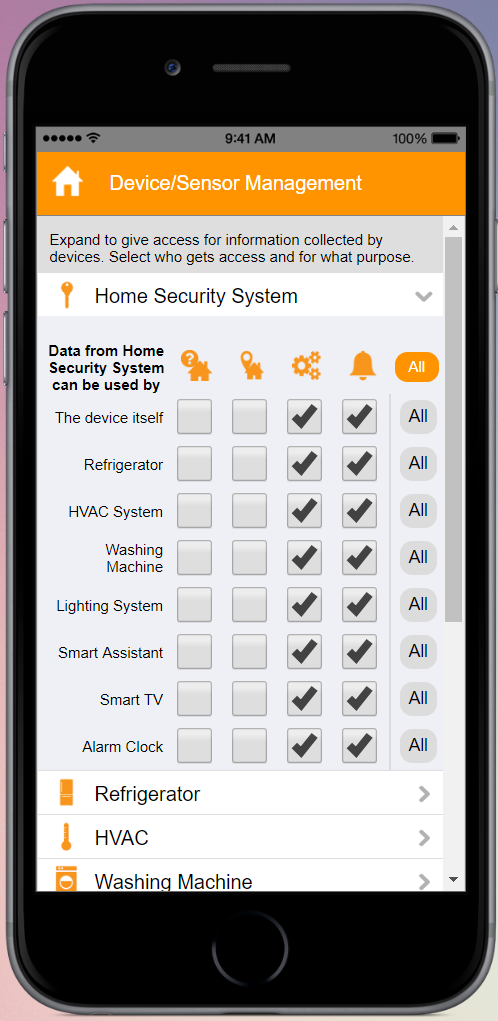
\includegraphics[height=2.8in]{figures/ui2sd4.png}
	\end{subfigure}%
	~~~~~
	\begin{subfigure}[t]{0.2\textwidth}
		\centering
		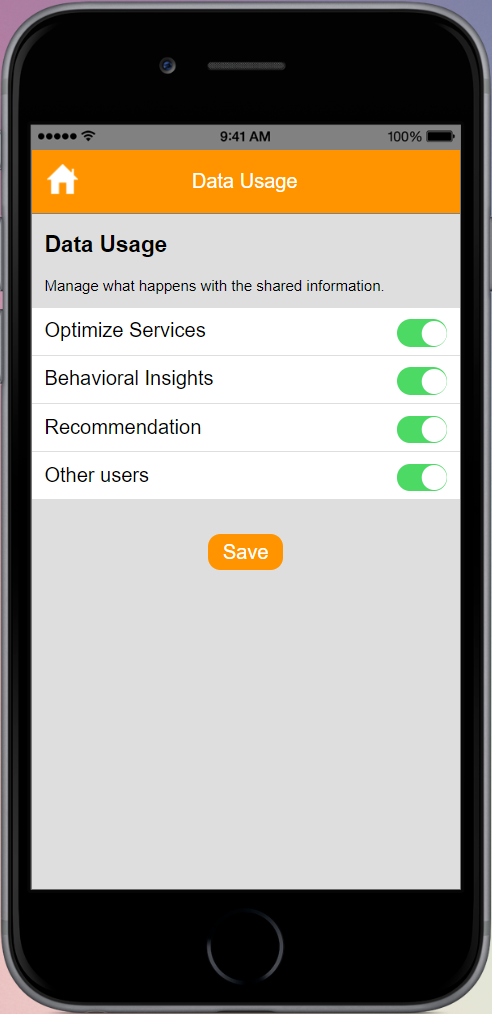
\includegraphics[height=2.8in]{figures/ui2sd5.png}
	\end{subfigure}%
	\caption{User Interface 2 with Smart Default}
	\label{fig:ui2SD}
\end{figure}

Figure~\ref{fig:ui1Profiles} shows the experimental condition --- UI1:Smart Profiles.
\begin{figure}[htb]
	\centering
	\begin{subfigure}[t]{0.2\textwidth}
		\centering
		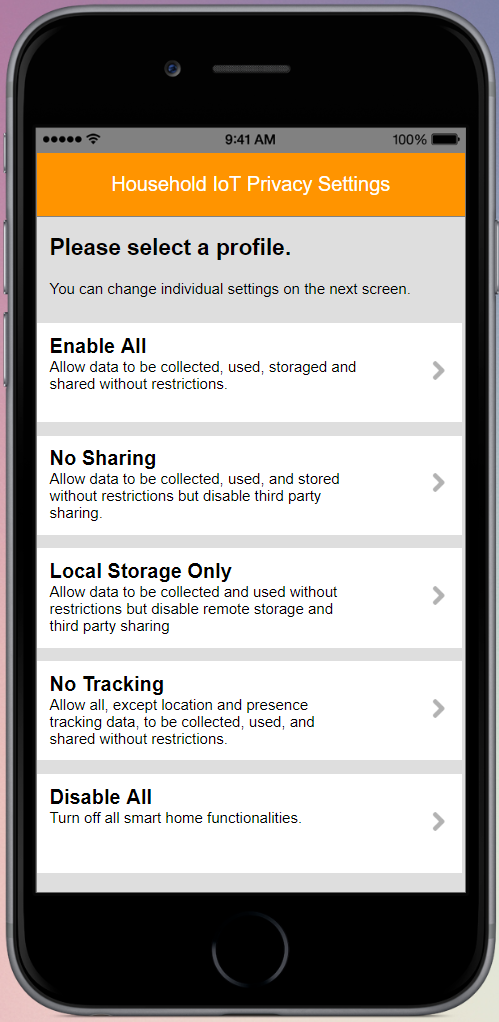
\includegraphics[height=2.8in]{figures/ui1sp1.png}
	\end{subfigure}%
	~~~~~
	\begin{subfigure}[t]{0.2\textwidth}
		\centering
		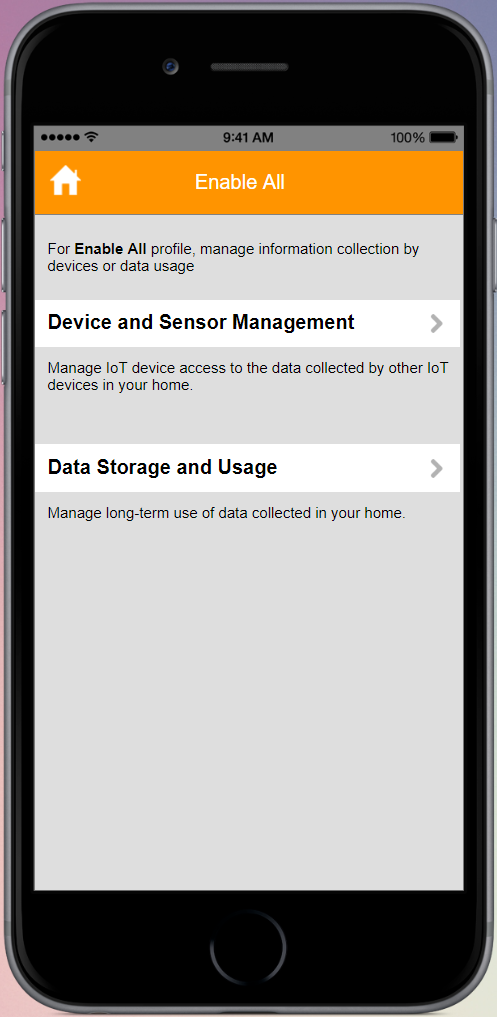
\includegraphics[height=2.8in]{figures/ui1sp2.png}
	\end{subfigure}%
	~~~~~
	\begin{subfigure}[t]{0.2\textwidth}
		\centering
		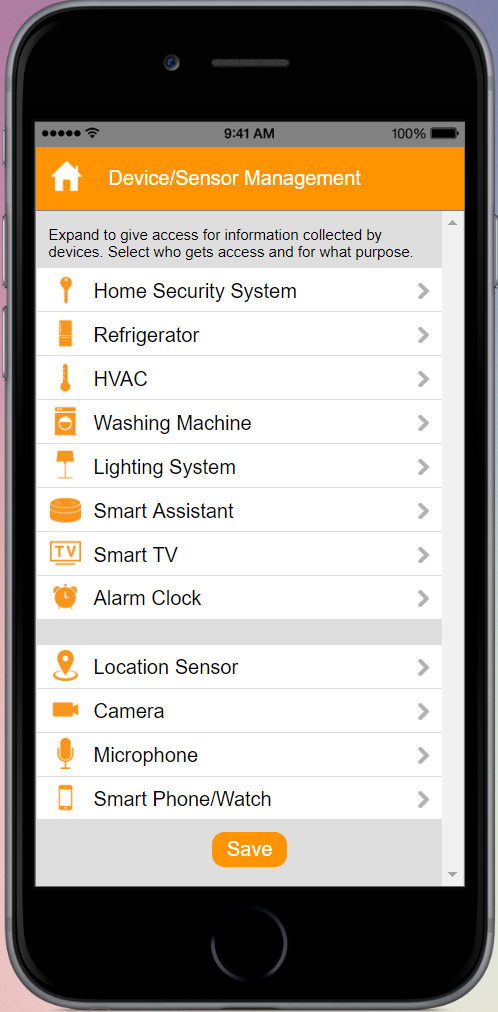
\includegraphics[height=2.8in]{figures/ui1sp3.png}
	\end{subfigure}%
	~~~~~
	\begin{subfigure}[t]{0.2\textwidth}
		\centering
		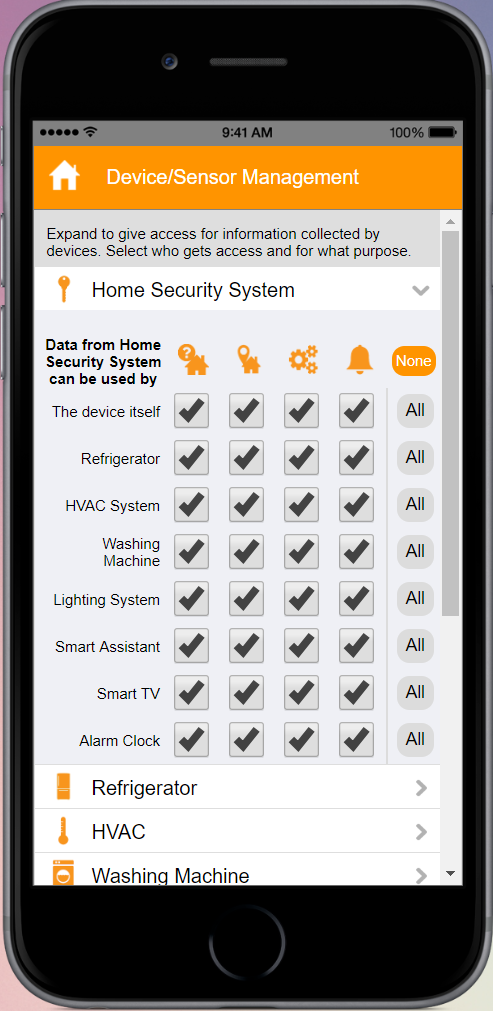
\includegraphics[height=2.8in]{figures/ui1sp4.png}
	\end{subfigure}%
	~~~~~
	\begin{subfigure}[t]{0.2\textwidth}
		\centering
		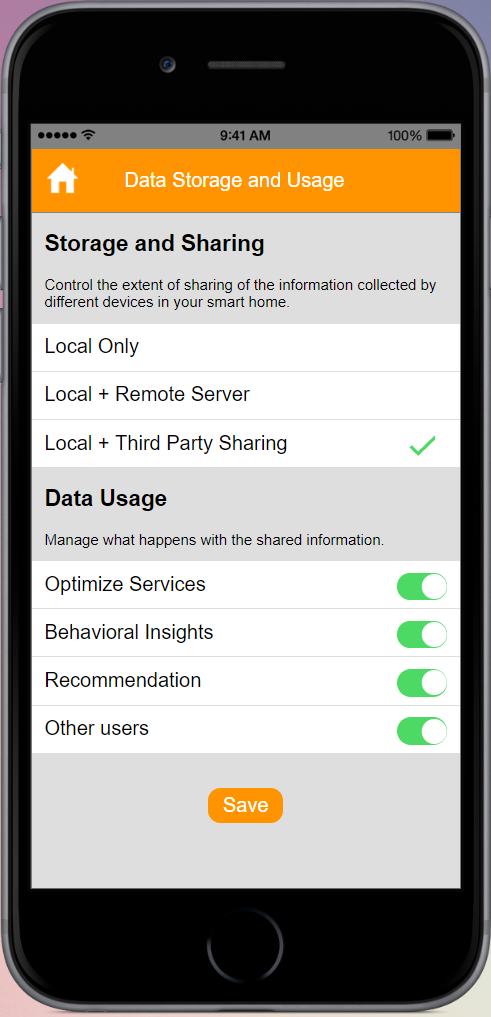
\includegraphics[height=2.8in]{figures/ui1sp5.png}
	\end{subfigure}%
	\caption{User Interface 1 with Smart Profiles}
	\label{fig:ui1Profiles}
\end{figure}

Figure~\ref{fig:ui2Profiles} shows the experimental condition --- UI2:Smart Profiles.
\begin{figure}[htb]
	\centering
	\begin{subfigure}[t]{0.2\textwidth}
		\centering
		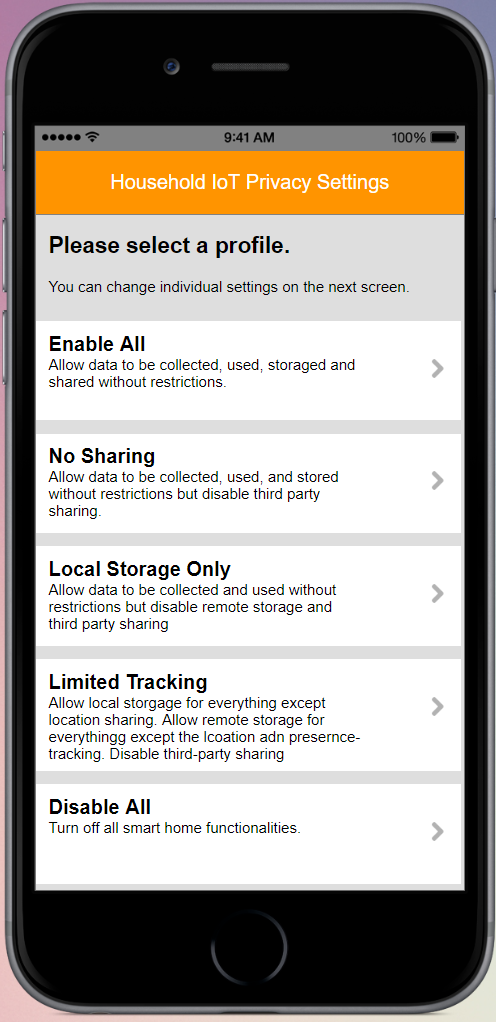
\includegraphics[height=2.8in]{figures/ui2sp1.png}
	\end{subfigure}%
	~~~~~
	\begin{subfigure}[t]{0.2\textwidth}
		\centering
		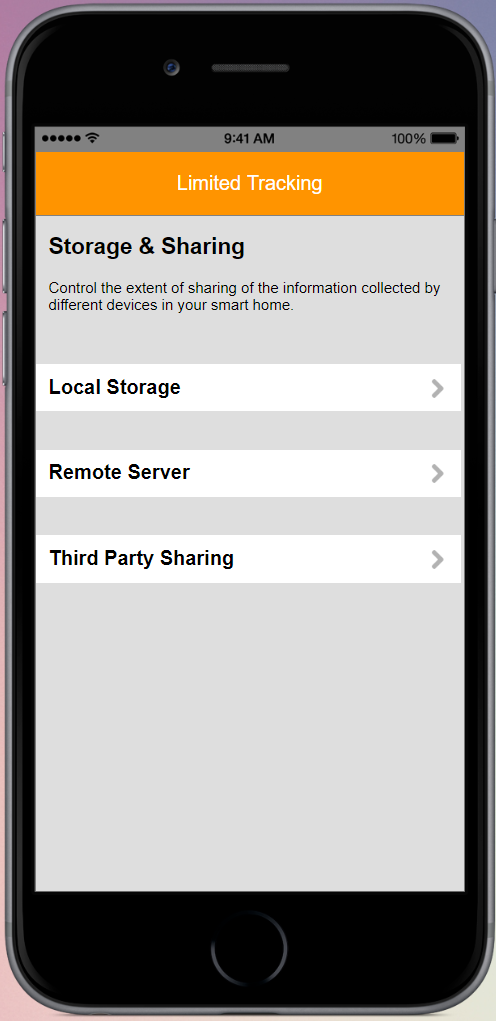
\includegraphics[height=2.8in]{figures/ui2sp2.png}
	\end{subfigure}%
	~~~~~
	\begin{subfigure}[t]{0.2\textwidth}
		\centering
		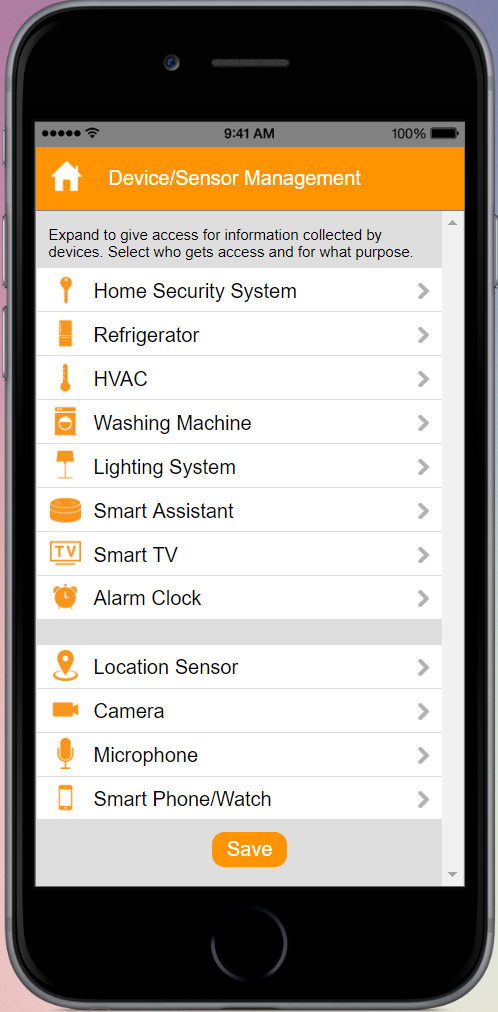
\includegraphics[height=2.8in]{figures/ui1sp3.png}
	\end{subfigure}%
	~~~~~
	\begin{subfigure}[t]{0.2\textwidth}
		\centering
		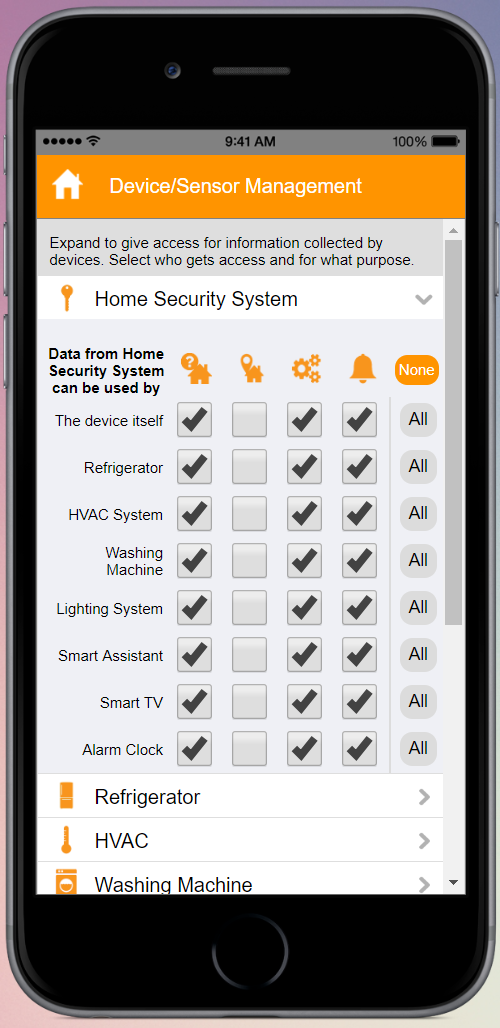
\includegraphics[height=2.8in]{figures/ui2sp4.png}
	\end{subfigure}%
	~~~~~
	\begin{subfigure}[t]{0.2\textwidth}
		\centering
		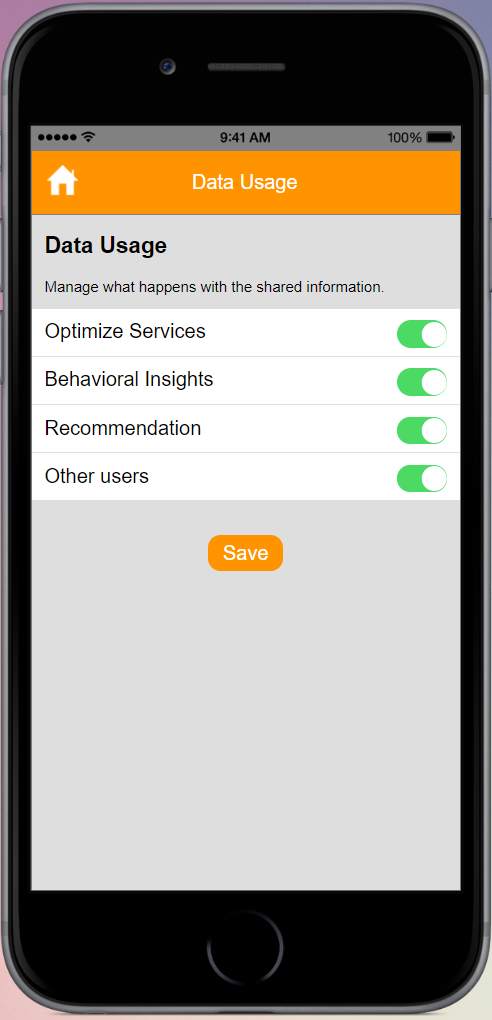
\includegraphics[height=2.8in]{figures/ui2sp5.png}
	\end{subfigure}%
	\caption{User Interface 2 with Smart Profiles}
	\label{fig:ui2Profiles}
\end{figure}

\subsection{Participants}
A power analysis shows that 400 participants will be needed for this study. In the study, all participants will be recruited via Amazon Mechanical Turk. After the study, each participant that successfully finishes the study and passes the attention check will be compensated \$1.5 dollars.

%To identify suitable participants, we will have screening questions on the recruitment ad:
%1). Do you currently have a household IoT device?
%2). Have you ever changed your privacy-settings of your household IoT devices?
%Participants will be enrolled in the study only if they meet all the screening criteria.



\subsection{Measurements}\label{subsection:measures}
A post-test survey questionnaire will be constructed to measure users' experience using our privacy-setting interfaces. The questionnaire will include three groups of questions. As shown in Figure~\ref{fig:uimodel}, the orange color items are experience (i.e. satisfaction with the system); the green color items are \textit{Subjective System Aspects} (SSA), including Perceived usefulness, Perceived easy of use, perceived privacy threats, perceived control); the blue color items are the personal/situational characteristics (General privacy concerns, Data Collection Concerns, Knowledge, Rational Decision Style, and Emotional Decision Style), the yellow color items are the experimental conditions (Interface Complexity and Profile Complexity). All items are adapted from previous published studies with minor modifications in wording to accommodate the IoT privacy-setting context. Each item will be measured on five-point Likert scales with 1 being "strongly disagree" to 7 being "strongly agree". All the items of the questionnaire are shown in Appendix.
\begin{figure}
	\centering
	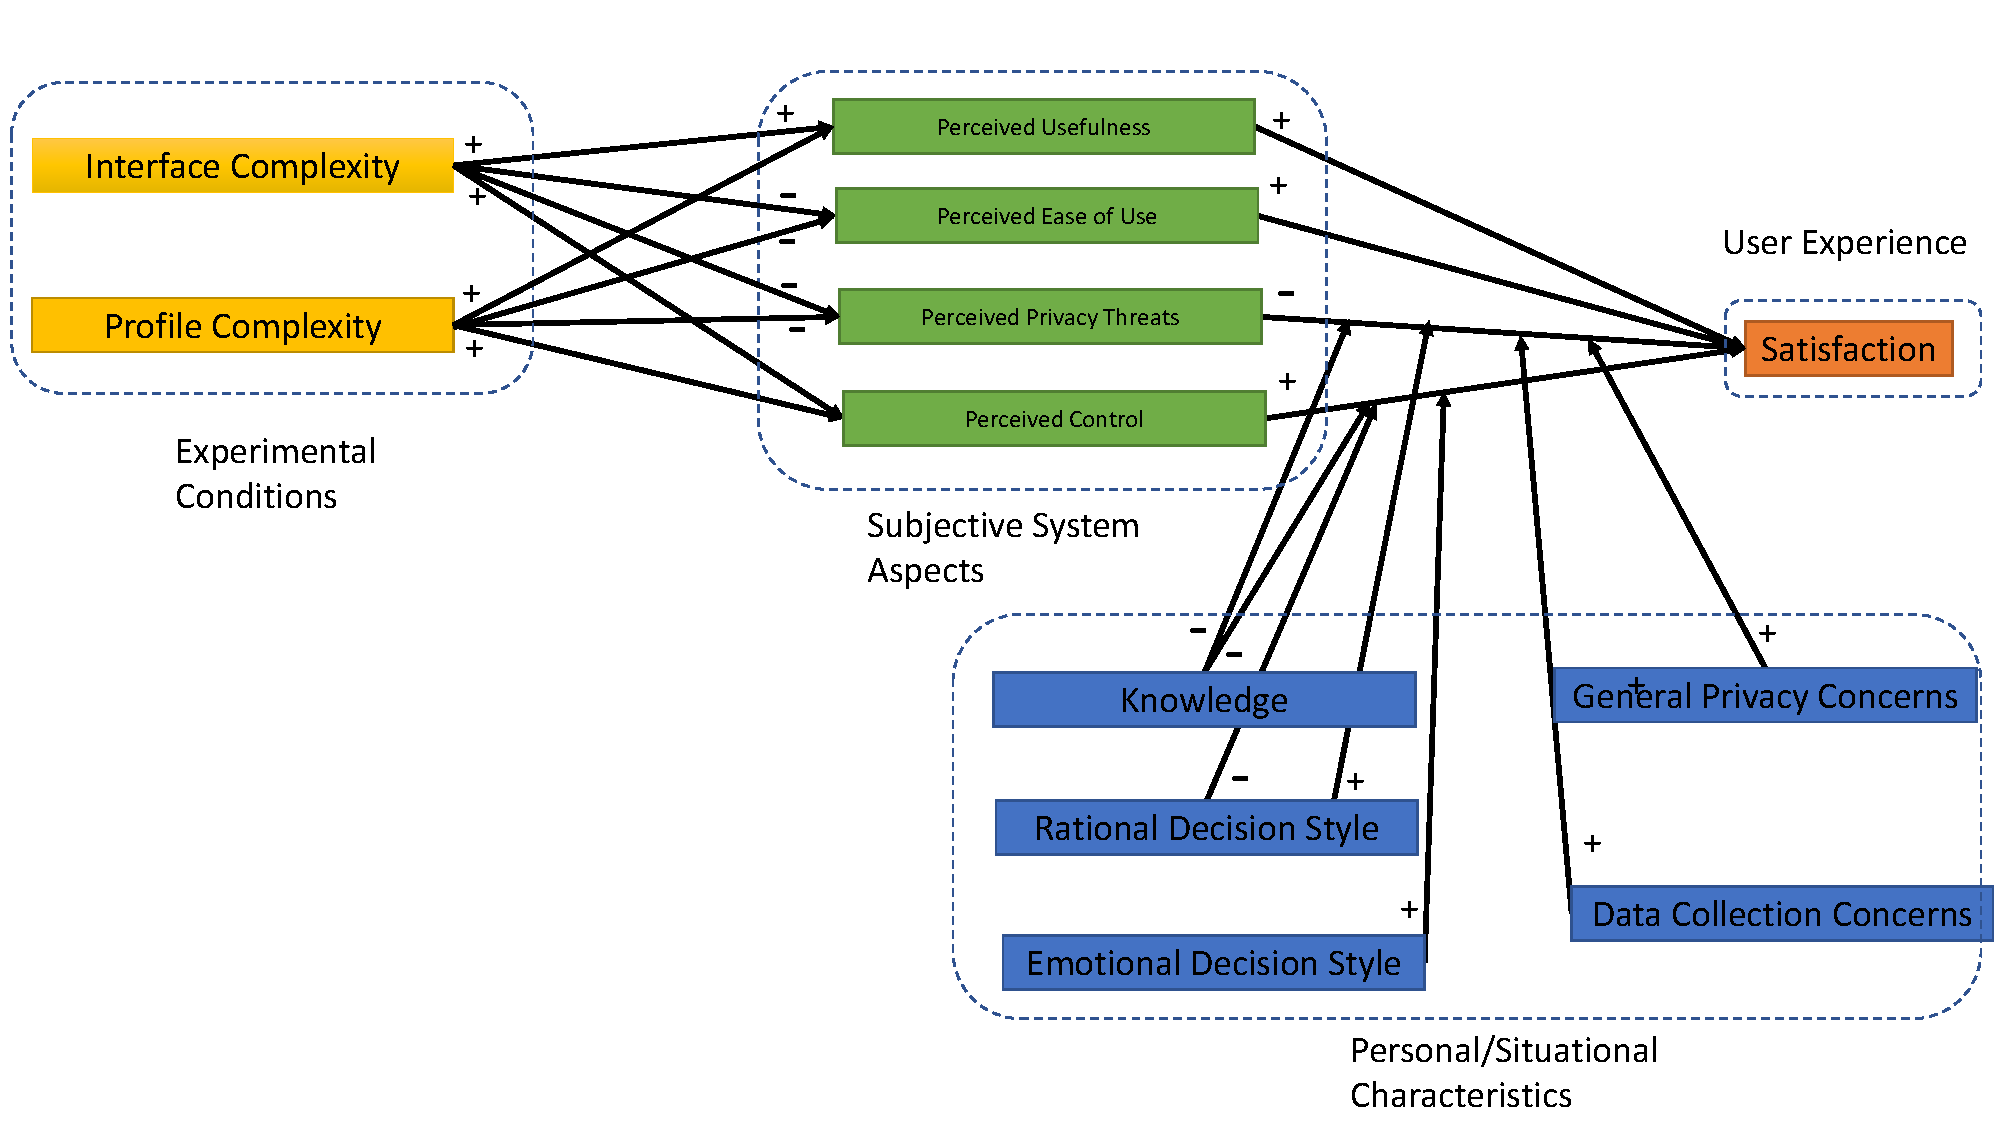
\includegraphics[width=\textwidth]{figures/uimodel.pdf}
	\caption{Expected Structural Model for Proposed User Study}
	\label{fig:uimodel}
\end{figure}

\subsection{Procedure}
During the user study~\footnote{The user study url can be found here: http://yyhe.people.clemson.edu/uistudy/}, the users will first be welcome with brief introduction of the experimental instructions, as shown in Figure~\ref{fig:us1}). We explicitly introduce that the goal of this study is to test a new Smart User Interface for Household IoT users.

\begin{figure}
	\centering
	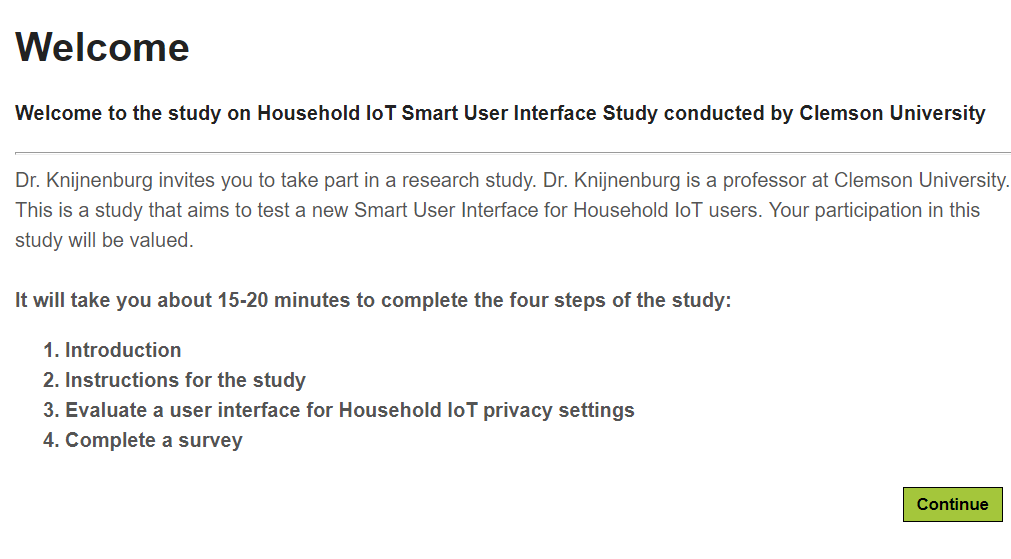
\includegraphics[width=0.85\textwidth]{figures/userstudy1.png}
	\caption{Experiment Welcome and Introduction Page}
	\label{fig:us1}
\end{figure}

Then the participants will be shown a consent form, as shown in Figure~\ref{fig:us2}.
\begin{figure}
	\centering
	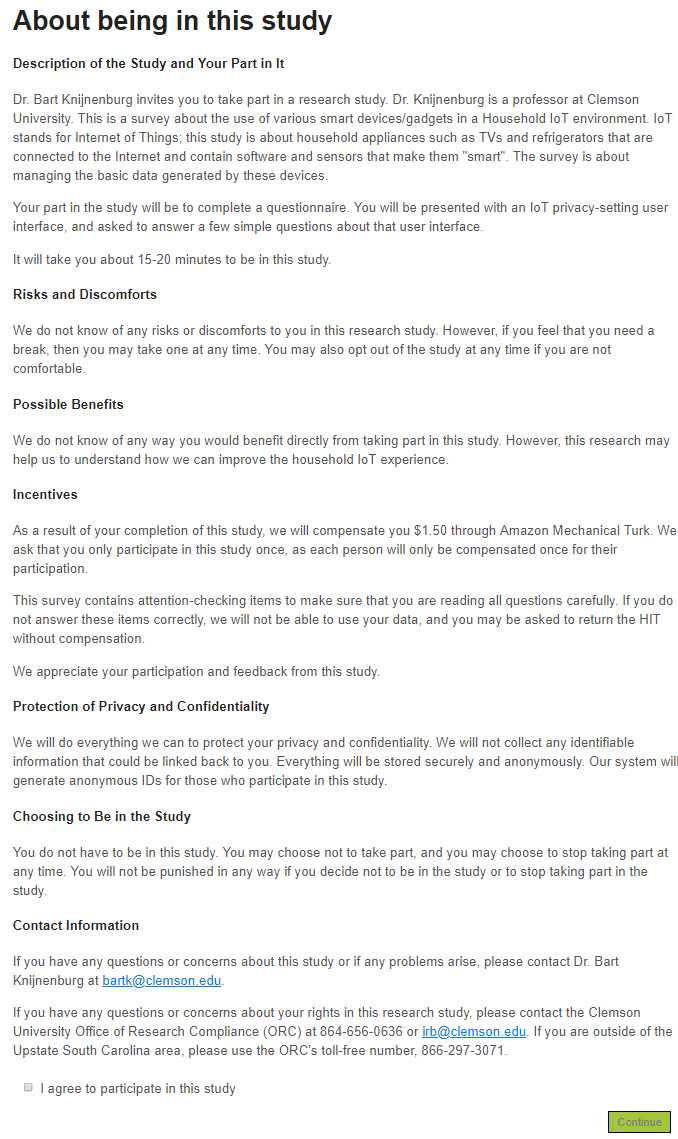
\includegraphics[width=0.8\textwidth]{figures/userstudy2.png}
	\caption{User Consent Form}
	\label{fig:us2}
\end{figure}

After signing the consent form, participants will be educated with the concept of the household IoT devices that appearing in this study, corresponding to the `Who' and `What' parameters of an IoT scenario, as shown in Figure~\ref{fig:us3}. This introduction to the household IoT contains figures, text, and audio information. After the introduction, participant will be given an example scenario to further understand the context of our study. Attention checks will also be given here to make sure the participants have paid attention to the explanations.
\begin{figure}
	\centering
	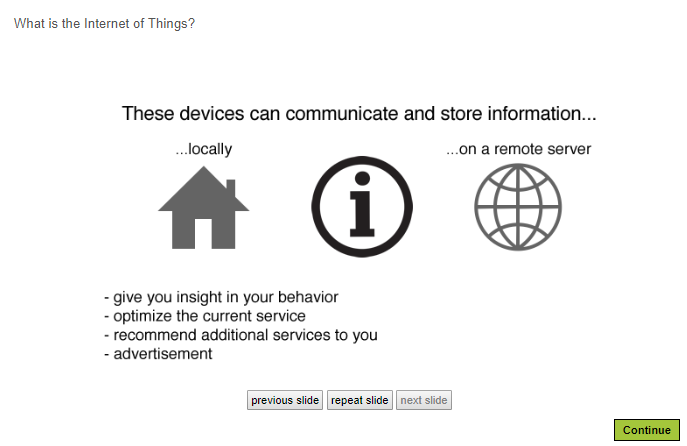
\includegraphics[width=\textwidth]{figures/userstudy3.png}
	\caption{Introduction to Household IoT}
	\label{fig:us3}
\end{figure}

After above procedures, one out of the 8 user interfaces will be randomly chosen for each participants. Participants need to go through the whole interface to see if the preset privacy settings is suitable for them, and make necessary changes to accommodate their actual privacy demands. All these changes will be recorded to compared with the preset settings for further analysis purpose. 

Next, the participants will be give a survey questionnaire discussed in Section~\ref{subsection:measures}.

After the user study is finished, We will first use \textit{confirmatory factor analysis} to clean up the items and then use \textit{linear mixed effects regression} to analyze the effect of the independent variables on the subjective system aspects, and further mediation effect on the user experience. We also wonder how the personal/situational characteristics affect the user experience.


\section{Expected Results}
In this section, we present our hypothesis on the expected results.

\subsection{Interface Complexity and SSA}
Compared to UI1, UI2 has more granularity when setting on different storage. In UI1, users can only configure all the privacy-settings to be the same for the three different types of storage (Local, Remote, and Third-party sharing), while they can configure those setting for each type of storage differently in UI2. Brandimarte et al. demonstrate that users perceive more control when privacy controls are more granular~\cite{brandimarte2013misplaced}. Therefore, we hypothesize the following:
\theoremgroup
\begin{theorem}
	Users that use UI2 will perceived  a higher control compared to users that use UI1.
\end{theorem}

Since more granular controls allow users to set their privacy settings to a level that better reflects their privacy preferences, this addition control may increase the perceived usefulness~\cite{tang2012implications, al2016modeling}. Therefore, we hypothesize the following:
\begin{theorem}
	Users that use UI2 will perceived a higher usefulness compared to users that use UI1.
\end{theorem}

Similarly, more fine-grained control may reduce users' perceived privacy threats. Tang et al. (2012) found that users of a finer-grained settings interface were more comfortable with their privacy settings. Therefore, we hypothesize the following:
\begin{theorem}
	Users that use UI2 will perceived a lower privacy threats compared to users that use UI1.
\end{theorem}

Research has shown that increasing the control often introduces choice overload issues~\cite{iyengar2000choice, schwartz2004paradox, acquisti2005privacy, acquisti2007can}, which makes it more difficult and time-consuming for users to accurately their privacy settings~\cite{madejski2012study, sadeh2009understanding}. Therefore, we hypothesize the following:
\begin{theorem}
	Users that use UI2 will perceived a lower ease of use compared to users that use UI1.
\end{theorem}

\subsection{Profile Complexity and SSA}
In term of profile complexity, we have four different levels of experimental conditions. These different default/profile conditions map to users' ``preference fit". ``Smart profiles" provide the users more pre-configured option to choose from, leading to a better preference fit than the ``smart default" with only single ``smart" option provided, which in turn has a better fit than Everything-Off/Everything-On defaults. This addition freedom of choice and possible increased preference fit may increase the perceived control and perceived usefulness. Therefore, we hypothesize the following:
\theoremgroup
\begin{theorem}
	Controlling other conditions, ``smart profiles" interfaces will have the highest perceived control, followed by ``smart default". Everything-Off and Everything-On defaults will have the lowest perceived control.
\end{theorem}
\begin{theorem}
	Controlling other conditions, ``smart profiles" interfaces will have the highest perceived usefulness, followed by ``smart default". Everything-Off and Everything-On defaults will have the lowest perceived usefulness.
\end{theorem}

Similarly, the increased preference fit may increase the level that the pre-configured profiles better reflect the users' privacy preferences, which may reduce the perceived privacy threats. Therefore, we hypothesize the following:
\begin{theorem}
	Controlling other conditions, ``smart profiles" interfaces will have the lowest perceived privacy threats, followed by ``smart default". Everything-Off and Everything-On defaults will have the highest perceived privacy threats.
\end{theorem}

The introduced addition options in ``smart profiles" again may introduce choice overload problem compared to the ``smart default" and Everything-Off and Everything-On defaults. This may lead to a low perceived ease of use for ``smart profiles". Compared to Everything-Off and Everything-On defaults, ``smart defaults" are generated from machine learning analysis results. The higher accuracy of ``smart defaults" can arguably assure a lower manual changes that users would make to the system, leading to a higher perceived ease of use compared to Everything-Off and Everything-On defaults. Therefore, we hypothesize the following:
\begin{theorem}
	Controlling other conditions, ``smart default" interfaces will have the highest perceived ease of use, followed Everything-Off and Everything-On defaults. ``smart profiles" will have the lowest perceived ease of use.
\end{theorem}

\subsection{Personal/Situational Characteristics and SSA}
Based on TAM and UTAUT that have been discussed in Chapter~\ref{chapter:Relatedwork1}, perceived usefulness can be increased by the benefits and advantages gained from the technology. In our study, perceived usefulness suggests the users will find the Household IoT privacy-setting interfaces that we designed are useful. Research has shown that perceived usefulness is a significant predictor of the intention to use IoT services~\cite{coughlan2012exploring}. Therefore, we hypothesize the following:
\theoremgroup
\begin{theorem}
	Perceived usefulness will be positively associated with users' satisfaction with the system.
\end{theorem}

Similarly, the causal relationship between the perceived ease of use of setting interfaces and users' satisfaction with the system has been codsified in both TAM and UTAUT. Several research has also verified this causal relationship~\cite{gao2014unified, dong2017understanding, choi2016smartwatch}. Therefore, we hypothesize following:
\theoremgroup
\begin{theorem}
	Perceived ease of use of the privacy-setting interfaces will be positively associated with users' satisfaction with the system.
\end{theorem}

Perceived privacy threats measures the level of privacy threatening regarding data collection and control perceived by users when using the system. A higher perceived privacy threats will lead to a higher system-specific concern of privacy risks~\cite{knijnenburg2013persuasive, knijnenburg2014increasing}. Therefore, we hypothesize following:
\theoremgroup
\begin{theorem}
	Perceived privacy threats will be negatively associated with users' satisfaction with the system.
\end{theorem}

The effect of perceived privacy threats on the system satisfaction may be moderated by the General Privacy Concerns and Data Collection Concerns. Research has shown that the negative association between over-sharing threat and system satisfaction will be stronger for users with a high level of Interpersonal privacy concerns~\cite{knijnenburg2014increasing}. However, for people with low Privacy  Concerns, the increased threat may not result in a reduced satisfaction with the system~\cite{hann2007overcoming, krasnova2009investigating}. Therefore, we hypothesize following:
\begin{theorem}
	The negative association between perceived threats and system satisfaction will be stronger for users with a high level of general privacy concerns or data collection concerns.
\end{theorem}

The positive effect of perceived control on the system satisfaction has been verified by a few research~\cite{malhotra2004internet, madejski2012study}. Therefore, we hypothesize following:
\begin{theorem}
	Perceived control will be positively associated with users' satisfaction with the system.
\end{theorem}

Knowledge measures how much the users know about the smart home devices. Users with a high level of knowledge may have a high level of expectations in data collection and control. When these users are evaluating the satisfaction with the system, the high level of expectation may moderate the effect of perceived privacy threats and perceived control. Therefore, we hypothesize following:
\theoremgroup
\begin{theorem}
	The negative association between perceived threats and system satisfaction will be stronger for users with a high level of knowledge.
\end{theorem}
\begin{theorem}
	The positive association between perceived control and system satisfaction will be weaker for users with a high level of knowledge.
\end{theorem}

The rest hypothesis are related to the rational decision style and emotional decision style. To our knowledge, there is no research has been done in the IoT context yet regarding the effect of decision style on the effect of perceived privacy threats and perceived control. Even in our previous study discussed in Chapter~\ref{chapter:householdIoT}, we did not find a significant effect of rational or emotional decision style on the decision of contextual scenarios. Still, we make following hypothesis based on these thinking: 1) users with a high level of rational decision style make think more about concrete privacy risk, leading to more perceived privacy threats and less perceived control; 2) It may be easier for users with a high level of emotional decision style to think the system is complex, leading to a higher perceived control.
\theoremgroup
\begin{theorem}
	The negative association between perceived threats and system satisfaction will be stronger for users with a high level of rational decision style.
\end{theorem}
\begin{theorem}
	The positive association between perceived control and system satisfaction will be weaker for users with a high level of rational decision style.
\end{theorem}
\begin{theorem}
	The positive association between perceived control and system satisfaction will be stronger for users with a high level of emotional decision style.
\end{theorem}


